\chapter{Installation of the software}
%-------------------------------

\lettrine[lines=2]{D}{iva} is a software designed to run with any operating system (Microsoft Windows, Linux, Mac OS X). The main steps for the the installation are described in this chapter. A more detailed and up-to-date list of instructions is available on the Installation web page of \diva: \url{http://modb.oce.ulg.ac.be/mediawiki/index.php/Diva_installation}

%%while the Graphical User Interface (GUI) is presented in Section~\ref{sec:guiinstall}. Note that the GUI is not up-to-date.

\minitoc

\newpage

\section{Requirements}
%---------------------

The basic requirements to run \diva are:
\begin{enumerate}
\item A command-line interface. With Linux or Mac, the interface is directly available: it is the shell or terminal. With Windows, it is necessary to install a Unix-like environment such as Cygwin (\url{http://www.cygwin.com/}).
\item A Fortran 95 compiler, such as:
\begin{itemize}
\item gfortran (\url{http://gcc.gnu.org/wiki/GFortran}),
\item ifort (Intel\textsuperscript{\textregistered}, \url{http://software.intel.com/en-us/intel-compilers}),
\item pgf (Portland Group, \url{http://www.pgroup.com/}).
\end{itemize}    
\itzm The NetCDF library (\url{http://www.unidata.ucar.edu/software/netcdf/}) for Fortran.
\end{enumerate}

For a quick visualization of the results, a software able to read and display the content of a NetCDF file is recommended:
\begin{itemize}
\item ncBrowse (\url{http://www.epic.noaa.gov/java/ncBrowse/}, a Java application,
\item Ncview (\url{http://meteora.ucsd.edu/~pierce/ncview_home_page.html}), a visual browser, 
\item Panoply (\url{http://www.giss.nasa.gov/tools/panoply/}, the NASA data viewer for various data formats.
\end{itemize}


\section{Download and extraction of the archive}
%-----------------------------------------

Select a directory on your local disk where you want install the software and download the archive available at \url{http://modb.oce.ulg.ac.be/mediawiki/index.php/DIVA#How_to_get_the_code.3F}.

\begin{lstlisting}[style=Bash]
[charles@gher13 ~]$ cd Software/
[charles@gher13 Software]$ wget http://modb.oce.ulg.ac.be/mediawiki/upload/DIVA/releases/GODIVA_07_2012.tar.gz
\end{lstlisting}

Extract the archive and go in the main directory:
\begin{lstlisting}[style=Bash]
[charles@gher13 Software]$ tar -xvf GODIVA_07_2012.tar.gz
[charles@gher13 Software]$ cd GODIVA_07_2012/
\end{lstlisting}

The directory tree has the following structure: %\newpage 
\begin{lstlisting}[style=Bash]
[charles@gher13 GODIVA_07_2012]$ tree -d -L 2
.
|-- DIVA3D
|   |-- bin
|   |-- divastripped
|   `-- src
|-- Doc
`-- JRA4
    `-- Climatology

7 directories
\end{lstlisting}


\begin{itemize}
\item \directory{DIVA3D/bin} contains the executables generated by the code compilation. Pre-compiled executables for various operating systems are provided in the sub-folders.
\item \directory{DIVA3D/divastripped} is the main working directory at the 2D level. 
\item \directory{DIVA3D/src} contains the Fortran source code. This is where the compilation has to be done.
\item[]
\item \texttt{Doc} contains the link to publications. For \LaTeX users: you find the corresponding \BibTeX entries in the file \texttt{DivaPublications.bib}.
\item \directory{JRA4/Climatology} is the main working directory at the 3D and 4D levels.
\end{itemize}

%----------------------------------------------
\section{Generation of the binaries (executables)}
%----------------------------------------------

There are two possibilities to obtain the binaries: 
\begin{enumerate}
\item Compile the source code.
\item Copy the provided binaries.
\end{enumerate}
The second option is provided for cases where the compilation was not possible, mainly because to missing libraries (e.g., NetCDF). 

\subsection{Compilation\label{sec:compilation}}

Go in the source directory 
\begin{lstlisting}[style=Bash]
[charles@gher13 GODIVA_07_2012]$ cd DIVA3D/src/Fortran/
\end{lstlisting}
and edit the configuration file \file{divacompile\_options} for the compilation  according to your machine. 

\begin{verbatim}
# Name of the fortran compiler (ex: ifort,gfortran,pgi,...)
compiler=ifort
# Compilation flags
flags='-O3'
# Netcdf library
nclib=/usr/local/lib/netcdf3ifort/libnetcdf.a
...
\end{verbatim}

If your installation knows the \command{nc-config} command, you can use 
\begin{verbatim}
# Netcdf library
nclib=`nc-config --flibs`
\end{verbatim}

Then run the compilation script: 
\begin{lstlisting}[style=Bash]
[charles@gher13 Fortran]$ divacompileall
\end{lstlisting}
and check the content of the log file (\file{compilation.log}). You should obtain something similar to that:
\begin{verbatim}
Compilation time:  Thu Oct 25 14:21:54 CEST 2012
compiler:          ifort
compilation flags: -O3
Calc directory:       1/1   program compiled
Extensions directory: 12/12 programs compiled
Mesh directory:       9/9   programs compiled
NC directory:         3/3   programs compiled
PlPlot directory:     1/1   programs compiled
Util directory:       38/38 programs compiled
Pipetest directory:   1/1   program compiled
Stabil directory:     28/28 programs compiled
----------------------------------------------------------
TOTAL:                93/93 programs compiled
----------------------------------------------------------
Binaries are located in directory:
/home/charles/Software/GODIVA_07_2012/DIVA3D/bin
\end{verbatim}

\section{Direct copy of pre-compiled binaries}

If the compilation failed, go in the \directory{GODIVA\_07\_2012/DIVA3D/bin/} directory and copy directly the binaries available in the sub-directories. For example for Windos with the Cygwin tool:
\begin{lstlisting}[style=Bash]
[charles@gher13 bin]$ cp -f cygwin/* .
\end{lstlisting}

\section{Run tests}
%------------------

In the main working directory (\directory{GODIVA\_07\_2012/DIVA3D/divastripped}), run one the two available tests: \command{divatest} and \command{divabigtest}. 


\subsection{Basic test}

\command{divatest} creates basic input files (see Chapter~\ref{chap:general}) for details), performs a simple \diva execution and check if the pipes are supported in your operating system (O.S.). The output can be checked using any software for reading NetCDF files. In this case we use ncview (see Chapter~\ref{chap:postprocessing} for details and installation). 

\begin{lstlisting}[style=Bash]
[charles@gher13 divastripped]$ divatest
...
[charles@gher13 divastripped]$ ncview output/ghertonetcdf/results.nc
\end{lstlisting}
The results you obtain has to be similar to those of Fig.~\ref{fig:diva_test_results}.

\begin{figure}[H]
\centering 
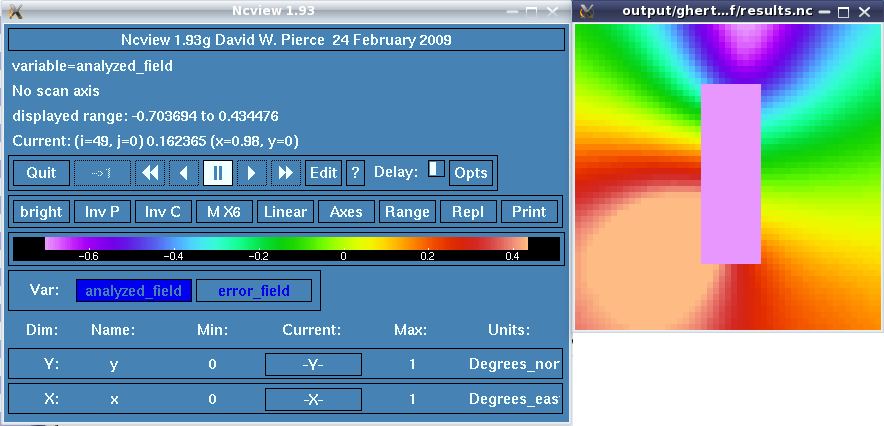
\includegraphics[width=.7\textwidth]{diva_test_results}
\caption{Results obtained with \command{divatest}.\label{fig:diva_test_results}}
\end{figure}

\subsection{Large-memory test}
%-----------------------------

\command{divabigtest} creates input files to simulate a case with a large number of data and a very fine mesh. Again, the results are viewable using the command:
\begin{lstlisting}[style=Bash]
[charles@gher13 divastripped]$ ncview output/ghertonetcdf/results.nc
\end{lstlisting}
and should be close to Fig.~\ref{fig:diva_bigtest_results}.

\begin{figure}[H]
\centering 
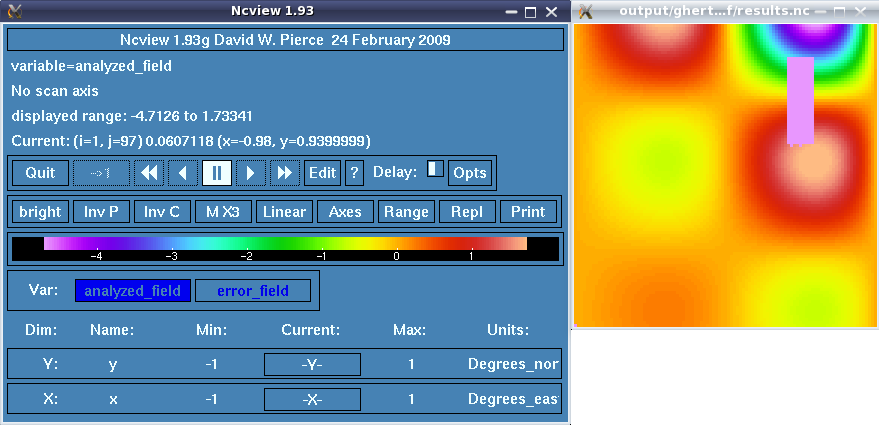
\includegraphics[width=.7\textwidth]{diva_bigtest_results}
\caption{Results obtained with \command{divabigtest}.\label{fig:diva_bigtest_results}}
\end{figure}



%\section{Command Line version}
%%-----------------------------
%
%This version is directly usable through a shell in the \texttt{divastripped} directory. 
%
%\begin{figure}[htpb]
%\centering
%\parbox{.65\textwidth}{
%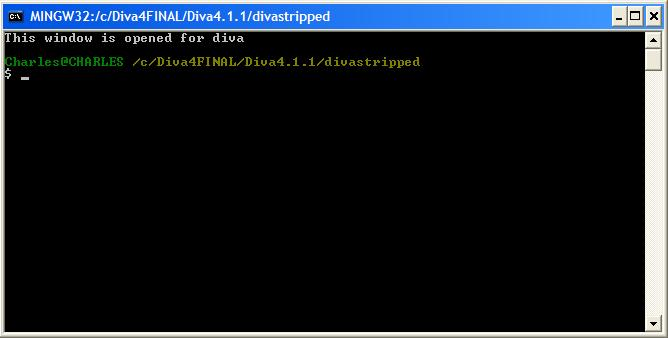
\includegraphics[width=.6\textwidth]{shell}
%}\parbox{.35\textwidth}{
%\caption{\texttt{Msys} shell.\label{shell}}
%}
%\end{figure}
%
%
%\subsection{Windows\label{windowsmsys}}
%%--------------------------------------
%
%You have two possibilities to have a Linux-like shell in your Windows environment:
%
%\begin{enumerate}
%
%\item \texttt{Cygwin}: it can easily be installed (or updated) from \url{http://www.cygwin.com/} by running \texttt{setup.exe} found there. \texttt{Cygwin} is a complete Linux-like environment, thus is recommended to Linux users.
%
%\item \texttt{Msys}: it constitutes the minimal environment under Windows. Its installation is described in the following. 
%
%\end{enumerate}
%
%\subsubsection{\texttt{Msys} installation}
%%-----------------------------------------
%
%If you need to install \texttt{Msys} on your computer:
%\begin{enumerate}
%\item Download the compressed file from\\ 
%\url{http://www.mingw.org/download.shtml}
%%\url{http://prdownloads.sourceforge.net/tcl/msys_mingw8.zip}
%\item Unzip \texttt{msys\_mingw8.zip} (or any recent version) in the chosen directory (let us assume in \texttt{C:/}).
%\item Open the \texttt{msys} shell (Fig. \ref{shell}) by double-clicking on the \texttt{msys} icon (MS-DOS command file) located in the \texttt{msys} folder.
%\end{enumerate}
%
%
%
%\subsection{Linux}
%%-----------------
%
%Under Linux, \texttt{msys} (or \texttt{cygwin}) installation is not required.
%
%
%
%\section{Executables\label{sec:executables}} 
%% ------------------------------------------
%
%
%The final step to achieve the \divainstallation consists in copying the pre-compiled versions of the executables (\texttt{*.a} files) corresponding to your system into \texttt{diva-\divaversion/bin}. They are provided in \texttt{diva-\divaversion/bin/Win32}, \texttt{diva-\divaversion/\-bin/\-Linux} and \texttt{diva-\divaversion/\-bin/\-SGI}.
%
%\example for Windows: open a shell in \texttt{diva-\divaversion} and type:\\
%\textcom{cp -fv ./bin/WIN32/*.a ./bin}
%
%

%
%\subsubsection{\tcltk}
%%---------------------
%
%As \tcltk\, is an interpreted language, it has not to be compiled. Modifications you may have made in \texttt{.tcl} files will be taken into account once you will have launched the \diva GUI.  
%
%
%
%\section{Creation of short-cuts}
%% -----------------------------
%
%Operations described in the present section are optional. The purpose is simply to have short-cut like\\ %\raisebox{-2mm}{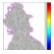
\includegraphics[height=.7cm]{logo_diva}} for GUI and\\ 
%\raisebox{-2mm}{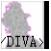
\includegraphics[height=.7cm]{logo_diva_cl}} for CL on your desktop.
%
%\subsection{Windows}
%%-------------------
%
%\begin{itemize}
%\item Copy \texttt{diva.ico}, \texttt{divacl.ico}, \texttt{diva.bat}, \texttt{divastripped.bat} and \texttt{.profile} (all found in \texttt{diva-\divaversion/\-inst\-all}) into the \texttt{msys} directory.
%
%
%\item Edit \texttt{.profile} and modify the third line according to your configuration.\\
%\example cd \textcom{c:/diva-\divaversion}
%
%\item With explorer, create short-cut to \texttt{msys/divastripped.bat} and move it to the desktop.
%
%\item Right-click on the desktop-shortcut-Properties:\\
%    in General: use \texttt{diva-\divaversion\, CL} instead of shortcut \ldots as text for the CL version,\\
%    in Shortcut: change icon, browse to \texttt{msys} and chose \texttt{divacl.ico}.
%    
%\end{itemize}
%
%
%%\subsection{Linux}
%%%-----------------
%%\begin{itemize}
%%\item Right-click on your desktop and select \textsl{Create launcher},
%%\item Type =  application,\\
%%name = DIVA (as you wish),\\
%%command = path to the \texttt{wish} executable + path to \texttt{main.tcl}.
%%\item In permission: allow executing file as program.
%%\end{itemize}
%
%
%
%\section{Run a test case}
%% -----------------------
%
%Now that everything is installed, we suggest you to run one of the test case provided in the sub-folders of \texttt{examples}. To this end, simply copy the files into the \texttt{divastripped/input/} directory (for example using command \texttt{divaload}, described in Sect. \ref{sec:divaload}). Open a shell, go in \texttt{./divastripped} and type \textcom{divadress}. If the process is not interrupted, our installation has been done properly. If not, a cause of the problem may be the executable: you may have to recompile the source, as described in Sec. \ref{sec:compilation}.
%
%
%\btips
%When working under Unix, you may have to convert the compilation script (\texttt{divacompile}) and the \textsl{batch} files (files with a name starting with \texttt{diva*} and file \texttt{dbdb2diva} located in \texttt{diva-\divaversion/divastripped}). 
%
%To perform the conversion, use the command \textcom{divados2unix} \footnote{This script uses \texttt{dos2unix}, which should be available within your \texttt{msys} or \texttt{cygwin} distribution.} provided in the \texttt{install} directory.
%\etips
%
%
%\btips
%Depending on the O.S. you have, the command \texttt{dos2unix} may behave differently. In some cases, running \texttt{dos2unix} twice will return you the original file (\textit{i.e.} the first time will convert the file to \texttt{unix}, the second one to \texttt{dos}). In that case you have to specify an option, such as
%
%\textcom{dos2unix -U}
%
%Hence, in case of doubt it is useful to have a look at the \texttt{dos2unix} command description for your system.
%\etips
%
%%\section{PlPlot library}
%%% ----------------------
%%\hypertarget{PLPLOT}{}
%%The PlPlot library is a set of Fortran routines that allow you to obtain graphical outputs without resort to external softwares, such as \matlab\, or NcView. Her is the procedure for the installation:
%%
%%\begin{enumerate}
%%
%%\item download the most recent version of PlPlot from\\
%%\url{http://plplot.sourceforge.net/}
%%
%%\item uncompress and unpack the archive \texttt{plplot-5.7.1.tar.gz}
%%
%%\begin{listevide}
%%\item \textcom{gunzip plplot-5.7.1.tar.gz}
%%\item \textcom{tar xvf plplot-5.7.1.tar.gz}
%%\end{listevide}
%%
%%\item in the directory \texttt{plplot-5.7.1}, type:
%%
%%\begin{listevide}
%%\item \textcom{./configure --prefix=MYPREFIX}, where MYPREFIX stands for the installation prefix (\example \texttt{/usr/local/plplot}) 
%%\item \textcom{make}
%%\item \textcom{make install}
%%\end{listevide}
%%
%%\item in the directory MYPREFIX/share/plplotVERSION/examples, type:
%%\begin{listevide}
%%\item \textcom{make}
%%\item \textcom{./plplot-test.sh} to see some examples.
%%\end{listevide}
%%
%%The complete installation procedure is described in the file \texttt{INSTALL}.
%%
%%\end{enumerate}
%
%

%\section[Installation checking]{Installation checking \expert}
%%-----------------------------------------
%
%This part is quite technical and is not essential for further use of the software. In directory \texttt{diva-\divaversion/install/} you find a series of tools allowing you to perform an elaborated check of your installation by comparing results of \diva executions with your installation with reference outputs. 
%
%Additional information can be found in \texttt{diva-\divaversion/install/README}.
%
%
%\subsection{\texttt{divamakecheck}}
%%----------------------------------
%
%Apply analysis on test cases listed in \texttt{divachecklist} and compare the results with references by applying \texttt{divacomp}.
%The command\\
%\texttt{divamakecheck -generate}\\
%will create new reference fields for later comparisons. Only developers shall use the \texttt{-generate} option.
%
%\subsection{\texttt{divacomp}}
%%-----------------------------
%
%Compare \texttt{ascii} output files generated by a \diva run with reference files provided with the distribution. Results of the comparison are written in \texttt{check.log}.
%
%
%\subsection{\texttt{divados2unix}}
%%---------------------------------
%
%Apply the conversion from dos-like to unix-like line endings on every \diva\texttt{ascii} file and set the permissions of the executables (\texttt{*.a} files) to 755. 
%
%
%
%
